%!TEX root = ../report.tex

\section{Kraft}

\subsection{Beispiele}
\begin{itemize}
    \item einmalig maximale Kraft (Gewichtheben)
    \item schnell und viel Kraft (Ringen, Hochsprung)
    \item Kraft aufrecht erhalten (Brücke)
\end{itemize}

\subsection{Anatomische Grundlagen}

\begin{wrapfigure}{r}{0.5\textwidth}
  \begin{center}
    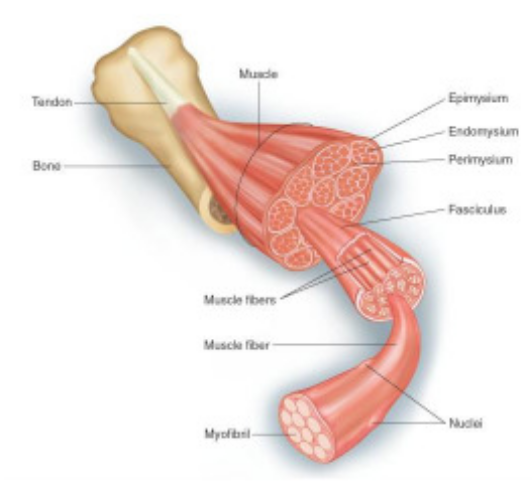
\includegraphics[width=0.48\textwidth]{pictures/muskeln}
  \end{center}
\end{wrapfigure}

\begin{itemize}
    \item grundsätzlich drei Komponenten: Muskel, Sehne, Knochen
    \item Muskel bestehen aus:
    \begin{itemize}
        \item Muskelfaserbündel
        \item Muskelfaser
        \item Myofibrille
        \item Sarkomer
        \item Aktin-Myosin
    \end{itemize}
\end{itemize}

\subsection{Aktionsformen der Muskeln}

\begin{tabular}{|c|c|c|c|}
 \hline
Kontraktionsform & Arbeitsweise & Ansatz / Ursprung & Beispiel Liegestütze \\ \hline \hline
konzentrisch & überwindend & Wird kleiner & Von Boden in Stütz \\ \hline
exzentrisch & nachgebend & Wird größer & Von Stütz auf Boden \\ \hline
isometrisch & haltend & Bleibt gleich & Halten des Stützes \\ \hline
\end{tabular}

\subsection{Struktur der Kraft}

Sportartspezifische Kraft = Kraftfähigkeiten + Technik

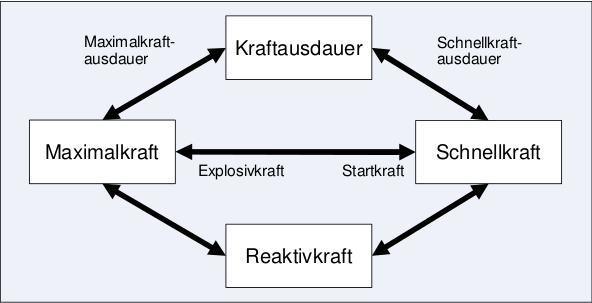
\includegraphics[width=0.8\textwidth]{pictures/kraftstruktur}

\subsection{Determinanten der Kraft}
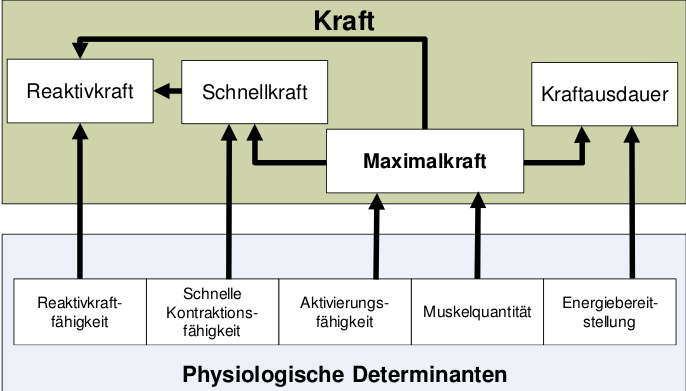
\includegraphics[width=0.8\textwidth]{pictures/kraft_determinanten}

\begin{wrapfigure}{R}{0.5\textwidth}
  \begin{center}
    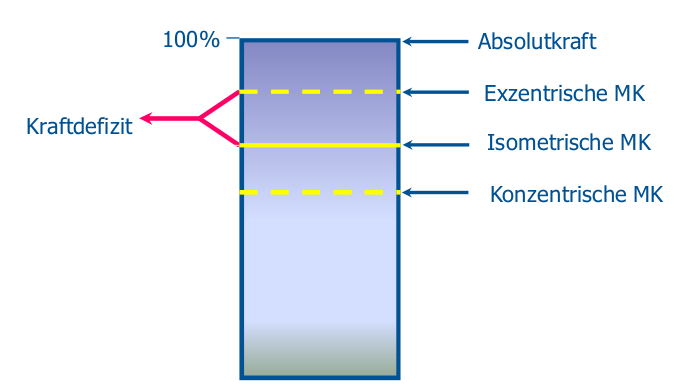
\includegraphics[width=0.48\textwidth]{pictures/maximalkraftvarianten}
  \end{center}
\end{wrapfigure}

\subsection{Maximalkraft}

\begin{itemize}
    \item Definition: Maximalkraft ist die höchstmögliche Kraft, die vom Nerv-Muskel-System willentlich gegen einen Widerstand erzeugt werden kann
    \item 1er-Maximum (1RM = 1 Repetition Maximum) = konzentrische Maximalkraft über volle Bewegungsamplitude
    \item Relativkraft = 1RM / Körpergewicht
    \item bestehend aus:
    \begin{itemize}
        \item Muskelquerschnitt \& Faserzusammensetzung
        \item Willkürliche Aktivierungsfähigkeit
    \end{itemize}
    \item Absolutkraft: Nur durch maximale elektrische Stimulation erreichbare Kraft. Willentlich nicht abrufbar.
    \item Kraftdefizit: $\frac{\text{Exzentrische MK} - \text{Isometrische MK}}{\text{Exzentrische MK}} \cdot 100 \%$
    \item in Praxis: Differenz zwischen isometrischer und exzentrischer MK
    \item Training:
    \begin{itemize}
        \item großes Kraftdefizit: willkürliche Aktivierungsfähigkeit verbessern
        \item kleines Kraftdefizit: Muskelquantität
    \end{itemize}
    \item
\end{itemize}

\subsection{Schnellkraft}

\begin{wrapfigure}{R}{0.5\textwidth}
  \begin{center}
    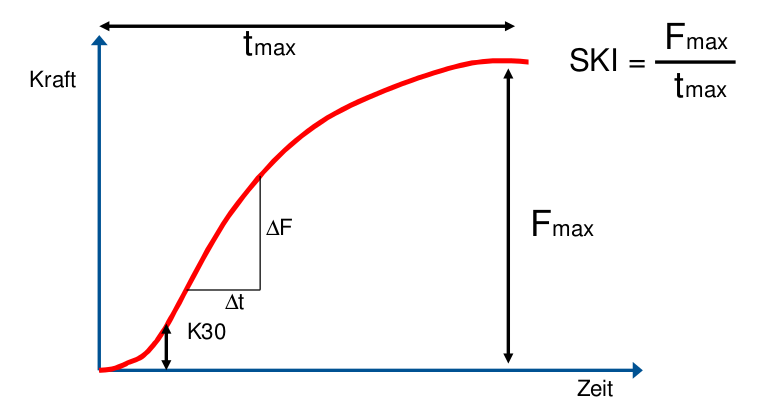
\includegraphics[width=0.48\textwidth]{pictures/kraftanstiegskurve}
  \end{center}
\end{wrapfigure}

\begin{itemize}
    \item Definition: Schnellkraft ist die Fähigkeit, einen möglichst großen Kraftstoß innerhalb einer zur Verfügung stehenden (kurzen) Zeit zu realisieren
    \item Teilaspekte:
    \begin{itemize}
        \item Startkraft (Fähigkeit sehr schnell Kraft zu entfalten, bsp: Boxen?)
        \item Explosivkraft (Fähigkeit großen/schnellen Kraftanstieg zu realisieren, bsp: Würfe, Stöße, Schüsse?)
        \item Dynamisches Kraftmaximum (Fähigkeit MK schnell zu realisieren, bsp: Ringen?)
    \end{itemize}
    \item Struktur der Schnellkraft: Maximalkraft + Schnelle Kontraktionsfähigkeit
    \item Schnelle Kontraktionsfähigkeit hängt ab von Muskelfaserzusammensetzung, Intermuskulärer und Intramuskulärer Koordination
\end{itemize}

